\chapter{Modulators}
The previous chapters wrote about the audio generators and manipulators. This section will take a look at some usefull modules which are used to modulate parameters within Odin 2.

Some of the modulators have hardwired functionalities in the synthesizer. However, the true potential of these (and the entire synth, really) lies in appling modulation from the \modmatrix.

\section{ADSR Envelopes}
\label{ADSR}
An ADSR Envelope provides a handy way of setting up a wide variety of curves like they can be observed in the timbre changes of physical instruments. ADSR Envelopes follow two basic signals: MIDI note-on and MIDI note-off. Depending on these, a curve is produced based on the four parameters \fat{Attack, Decay, Sustain} and \fat{Release}.

Odin 2 provides four of these Envelopes:

\begin{center}
    \includegraphics[width=0.4\textwidth]{graphics/ADSR_section.png}
\end{center}

The \fat{Amp Envelope} is hardwired to control the volume curve of the voice. This effect is not applied in the actual Amplifier module, but after the Distortion section (see Section \ref{routing}). Note that the Amp Envelope can still be used as a freely assignable modulation source in the \modmatrix. This Envelope is calculated for each voice independently.
\label{amp_env}

The \fat{Filter Envelope} is hardwired to modulate the frequencies of the various Filter modules in Odin 2. For this to take effect, the parameter "Filter Env" (see Section \ref{filters}) has to be enabled. The modulation by this envelope can be in either positive or negative direction. This Envelope is calculated for each voice independently.

The \fat{Mod Envelope} is a freely assignable modulation source. This Envelope is calculated for each voice independently.

The \fat{Global Envelope} is different from the other three Envelopes in that it exists only once for all voices. This can come in handy when you want the modulation not to diverge between voices.

To switch between the different Envelope modules, use their handles on top of the section:
\begin{center}
    \includegraphics[width=0.5\textwidth]{graphics/ADSR_handles.png}
\end{center}
Two envelopes are paired to occupy the same space. To acces the currently not visible Envelope, simply click on its name.

\begin{center}
    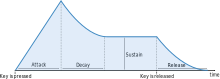
\includegraphics[width=\textwidth]{graphics/ADSR.png}
\end{center}

\audioparameter{Attack}{1}{1}{
    The Attack determines the time the Envelope takes from the start to the first peak.

    When playing the synth in Legato mode (see Section \ref{legato}), the attack section will start from the last value the Enveope from the previous voice produced. No matter the start height, the slope of the Attack will always be the same as if it started from zero.

    Using really short Attack times can introduce clicks into the sound, so it is advisable to have at least some attack for most situations.

    Note that unlike the Decay and Release sections, the Attack follows a linear curvature.
}

\audioparameter{Decay}{1}{1}{
    The Decay controls the time the Envelope will take to fall to the sustain value after the Attack reached its highest point. This curve will always start at the internal value one, and will always fall to the value specified by the Sustain parameter.

    The Decay section follows an exponential falling curvature.
}

\audioparameter{Sustain}{1}{1}{
    The Sustain determines the level that the Evelope will fall to after the Decay section. Note that the Sustain section will be active after Decay finished for as long as the MIDI-key is not released.
}

\audioparameter{Release}{1}{1}{
    The Release controls the time the Envelope will take to fall to zero after the MIDI-key was released. No matter what stage is currently active, once the key is released, the Envelope will jump right to the Release section immediately. The starting point for the falling curve will always be the last value that the Envelope produced. A finished Release section of the Amp Envelope gives the synthesizer the signal to end processing for this voice.

    The Release section follows an exponential falling curvature.
}

\audioparameter{ADSR Loop}{0}{1}{
    The loop parameter gives the option to start the Attack section again after the Decay is finished, thereby creating an LFO-type modulation source.
}

\section{Low Frequency Oscillators (LFOs)}
\label{LFOs}

\begin{center}
    \includegraphics[width=0.4\textwidth]{graphics/LFOs.png}
\end{center}

A Low Frequency Oscillator (LFO) is an Oscillator module which operates at frequencies below the human hearing range. They are therefore not suited for audio signal generation, but play a crucial role in slowly modulating parameters over time in synthesizers. Like with all Oscillators in Odin 2, waveforms and operation speeds can be controlled.

Odin 2 has four LFO modules: LFO1, 2 and 3 are available per voice. The fourth GlobalLFO exists only once for all voices. It can therefore be used to modulate all voices identically. The LFOs are also capable to act as a Sample \& Hold module. See the parameter "LFO Waveform" for details on how to activate it.

To switch between the different LFO modules, use their handles on top of the section:
\begin{center}
    \includegraphics[width=0.5\textwidth]{graphics/LFO_handles.png}
\end{center}
Two LFOs are paired to occupy the same space. To acces the one currently not visible , simply click on its name.

\audioparameter{LFO Freq}{1}{1}{
    Controls the speed of the oscillator. Depending on the parameter "LFO Sync", this is either a dial for continuous values in Hz, or a custom selector to sync the time to the beat. This selector allows for arbitrary fractions of the current host BPM, for example 3/16th notes:

    \begin{center}
        \includegraphics[width=0.18\textwidth]{graphics/LFO_sync.png}
    \end{center}

    Please note that a synced LFO does not keep track of the playback position of the DAW. The oscillator is still free-running, but the frequency is derived from host-BPM.
}

\audioparameter{LFO Sync}{0}{1}{
    Controls whether the LFO Freq is set by a knob in Hz or via the sync-time selector, syncing it to the host BPM.
}

\audioparameter{LFO Waveform}{0}{0}{
    Determines what waveform is used by the Oscillator. Available Waveforms are:

    \vspace{3mm}
    \begin{tabular}{| L{0.12\textwidth} | L{0.8\textwidth} |}
        \hline
        \includegraphics[width=0.1\textwidth]{graphics/LFO/sine.png}      &
        A sine wave\\
        \hline
        \includegraphics[width=0.1\textwidth]{graphics/LFO/saw.png}       &
        A falling sawtooth wave                                             \\
        \hline
        \includegraphics[width=0.1\textwidth]{graphics/LFO/triangle.png}  &
        A triangle wave\\
        \hline
        \includegraphics[width=0.1\textwidth]{graphics/LFO/square50.png}  &
        A pulse wave with pulse width 0.5\\
        \hline
        \includegraphics[width=0.1\textwidth]{graphics/LFO/square25.png}  &
        A pulse wave with pulse width 0.25\\
        \hline
        \includegraphics[width=0.1\textwidth]{graphics/LFO/square12.png}  &
        A pulse wave with pulse width 0.125\\
        \hline
        \includegraphics[width=0.1\textwidth]{graphics/LFO/peak.png}      &
        A waveform with a sharp peak in the middle\\
        \hline
        \includegraphics[width=0.1\textwidth]{graphics/LFO/SH.png}        &
        \fat{Sample \& Hold}: This is not a waveform, but sets the LFO to S\&H operation. Each time a cycle is complete, a new bipolar random value is generated, which is held for the entire cycle.\\
        \hline
        \includegraphics[width=0.1\textwidth]{graphics/LFO/pyram4.png}    &
        A pyramid shaped waveform with four discrete steps.\\
        \hline
        \includegraphics[width=0.1\textwidth]{graphics/LFO/pyram6.png}    &
        A pyramid shaped waveform with six discrete steps\\
        \hline
        \includegraphics[width=0.1\textwidth]{graphics/LFO/pyram8.png}    &
        A pyramid shaped waveform with eight discrete steps\\
        \hline
        \includegraphics[width=0.1\textwidth]{graphics/LFO/pyram12.png}   &
        A pyramid shaped waveform with twelve discrete steps\\
        \hline
        \includegraphics[width=0.1\textwidth]{graphics/LFO/stair3.png}    &
        A stair shaped waveform with three discrete steps\\
        \hline
        \includegraphics[width=0.1\textwidth]{graphics/LFO/stair4.png}    &
        A stair shaped waveform with four discrete steps\\
        \hline
        \includegraphics[width=0.1\textwidth]{graphics/LFO/stair6.png}    &
        A stair shaped waveform with six discrete steps\\
        \hline
        \includegraphics[width=0.1\textwidth]{graphics/LFO/stair8.png}    &
        A stair shaped waveform with eight discrete steps\\
        \hline
        \includegraphics[width=0.1\textwidth]{graphics/LFO/stair12.png}   &
        A stair shaped waveform with twelve discrete steps\\
        \hline
        \includegraphics[width=0.1\textwidth]{graphics/LFO/wavedraw1.png} &
        The waveform which was drawn in the WaveDraw Osc in slot 1 (See Section \ref{wavedraw})\\
        \hline
        \includegraphics[width=0.1\textwidth]{graphics/LFO/wavedraw2.png} &
        The waveform which was drawn in the WaveDraw Osc in slot 2 (See Section \ref{wavedraw})\\
        \hline
        \includegraphics[width=0.1\textwidth]{graphics/LFO/wavedraw3.png} &
        The waveform which was drawn in the WaveDraw Osc in slot 3 (See Section \ref{wavedraw})\\
        \hline
    \end{tabular}
}

\audioparameter{LFO Reset}{0}{1}{
    Resets the LFO to the beginning of the wave on note start.
}

\section{XY-Pad}
\label{xy}
\begin{center}
    \includegraphics[width=0.35\textwidth]{graphics/XY_pad.png}
\end{center}

The XY-Pad provides a convenient way to combine two independent modulation sources which can be intuitively modified with your mouse. Modulations set up with the XY-Pad often yield interesting and unpredicted sounds.

\audioparameter{XY-Pad X}{0}{1}{
    Controls the X-axis of the XY-Pad.
}

\audioparameter{XY-Pad Y}{0}{1}{
    Controls the Y-axis of the XY-Pad.
}

\section{Modwheel \& Pitchbend}
\label{wheels}

\begin{center}
    \includegraphics[width=0.15\textwidth]{graphics/wheels.png}
\end{center}

Modwheel and Pitchbend provide two basic modulation sources which can be found on most MIDI keyboards.

\audioparameter{Pitchbend}{0}{1}{
    Pitchbend allows you to easily transpose the sound of all Oscillators (See Chapter \ref{oscillators}). The amount of transposition is controlled by the parameter "Pitchbend Range" in semitones. Default is +/- 12 semitones.

    This control will automatically track all MIDI Pitchbend messages send to Odin 2 and update accordingly. 
    
    You can use the pitchbend as a modulation source as well.
}

\audioparameter{Pitchbend Range}{0}{0}{
    Controls how far Pitchbend modulates the pitch of the oscillators in either direction. Can be set to zero to use the Pitchbend as a pure modulation source for other parameters.
}

\audioparameter{Modwheel}{0}{1}{
    A freely assignable modulation source, which is also found on most MIDI keyboards. It is therefore a very common modulation source for expressive play.

    This control will automatically track all MIDI Modwheel messages (MIDI-CC 001) send to Odin 2 and update accordingly.
}